\section{模型评价}

  \subsection{模型优点}

    %\begin{figure}[htbp]
    %  \centering
    %  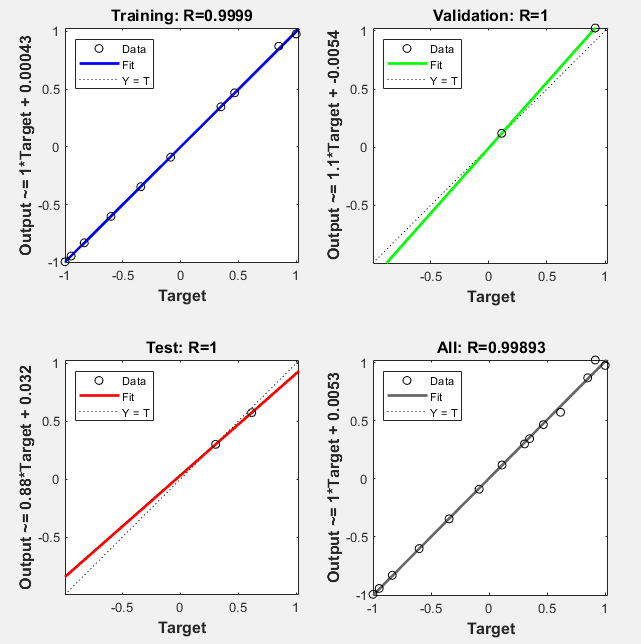
\includegraphics[width=0.618\paperwidth]{figures/muxinnihe.png}
    %  \caption{模型拟合相关系数 $\mathrm{R}$}
    %  \label{fig:muxinnihe}
    %\end{figure}

    \begin{table}[htb]
      \centering
      \caption{模型拟合结果}
      \begin{tabular*}{0.618\paperwidth}{@{\extracolsep{\fill}}ccccccc}
        \toprule[1.5pt]
        &隐含层节点数 && 训练次数 && $\mathrm{MES}$ &\\
        \midrule[1pt]
        &6 && 10 && 0.0060454 &\\
        \bottomrule[1.5pt]
      \end{tabular*}
      \label{tab:nihejieguo}
    \end{table}

    由上面两个图表可知\cite{zhangfaming2016}:
    \begin{enumerate}
      \item $\mathrm{BP}$ 神经网络模型的相关系数 $\mathrm{R}=0.99893$ ,十分接近 1,拟合效果十分理想。
      \item 训练次数较少,$\mathrm{BP}$ 神经网络能较快拟合。均方根误差 $\mathrm{MES}$ 非常的小且
      \item 同时预测平均相对误差较小,可以较好的预测碳排放量。
    \end{enumerate}
    
    此外,由问题求解可知:
    \begin{enumerate}
      \item 非常适合求解内部机制复杂、难以清晰暴露内部机理的问题
      \item 自我学习,能随数据不断改善自身。
    \end{enumerate}

  \subsection{模型缺点}
    \begin{enumerate}
      \item 样本数据较少,存在过拟合可能性。
      \item BP神经网络模型不能清晰的反应不同因素对碳排放量的影响程度。
      \item 模型不一定包括了所有影响因素。
    \end{enumerate}